\documentclass[a4paper]{llncs}

\usepackage[T1]{fontenc}

\usepackage{url}
\usepackage{amssymb}
\usepackage{subfigure}
\usepackage{verbatim} % for comment environment


\ifx\pdfoutput\undefined
\usepackage{graphicx}
\else
\usepackage[pdftex]{graphicx}
\fi

\graphicspath{{figures/}}

% \usepackage{pnml}
% \lstset{language=[structured]PNML,basicstyle=\ttfamily\small,commentstyle=\itshape,%
%   stringstyle=\itshape,keywordstyle=\underbar,% numberstyle=\tiny,%
%   stepnumber=5,showstringspaces=false,% numbers=left,%
%   % belowcaptionskip=\bigskipamount,
%   basewidth=.5em,escapechar=\$}


% \newcommand{\ignore}[1]{}

\title{
  ePNK Applications and Annotations:\\
  A Simulator for YAWL Nets%\thanks%
%  {Note that a short version of this paper has been presented at the workshop AWPN 2017
%   (Algorithms and Tools for Petri Nets), held in Kgs. Lyngby, Denmark, Oct. 19--20, 2017:
%   {\tt http://www2.compute.dtu.dk/\~{}ekki/conferences/AWPN-2017}}%
} 

\author{Ekkart Kindler}
\institute{Software Engineering Section, DTU Compute, Technical University of Denmark\\
\email{ekki@dtu.dk}
}

\begin{document}

\maketitle

\begin{abstract}

The \emph{ePNK} is an Eclipse based platform and framework for developing and
integrating Petri net tools and applications. 
% One of its core features is that
New types of Petri nets can be realized and plugged into the ePNK without any
programming by simply providing a model of the concepts of the new \emph{Petri net type}.
Moreover, the ePNK allows developers to customize the graphical appearance of
the features of a new Petri net type.

\begin{comment}
The main idea and features of the ePNK have been presented before. One important
aspect of the ePNK, however, has not been discussed yet: how to
realize new \emph{applications} for the ePNK and, in particular, how
to visualize the result of an application in the graphical editor of the ePNK
by so-called \emph{annotations}, and how the application can
use these annotations for interacting with the end user.

In this paper, we discuss how to implement an ePNK application
by the example of YAWL nets along with a simulator for them.
In addition, we discuss how annotations could be the basis
for an interchange format for analysis results of Petri nets.
\end{comment}

In this paper, we discuss how to implement \emph{applications}
for the ePNK, and how they can interact with the end user
by so-called \emph{annotations}. This is discussed by the example of
a simulator for YAWL nets.

{\bf Keywords:}
  Petri net tools,
  Framework,
  Petri Net Markup Language (PNML),
  Applications,
  Annotations.
\end{abstract}

% TODO: Plain style needs to be deleted in the final version
% \pagestyle{plain}

\section{Introduction}
\label{sec:intro}

% \nocite{HKea09,ISO-IEC:15909-2-2011, ePNKHome16}

The \emph{ePNK} is an Eclipse based platform and framework for developing and
integrating Petri net tools and applications. One of its core features is that
the ePNK can be easily equipped with new types of Petri nets:
they  can be realized and plugged into the ePNK without any
programming by providing a model of the concepts of the new type, the so-called
\emph{Petri net type definition} (\emph{PNTD}) as introduced for the
\emph{Petri Net Markup Language} (\emph{PNML}) \cite{HKea09,ISO-IEC:15909-2-2011}.
Moreover, the ePNK allows developers to customize how the features of a
new Petri net type are represented in the graphical editor of
the ePNK.

The main idea and features of the ePNK as a tool that fully supports
PNML have been presented before \cite{Kin11d,Kin12c}.
One important aspect of the ePNK, however, has not been discussed yet:
ePNK \emph{applications} and how to realize them. This, in particular,
includes visualizing the result of an application on top of the
Petri net in the graphical editor of the ePNK by using \emph{annotations},
and ePNK's mechanism for an application to interact with the end user
via annotations.

In this paper, we give an overview of the concepts of ePNK applications by discussing
the implementation of a simulator for YAWL nets \cite{vAtH05}. Moreover, we briefly discuss
how the ePNK's annotations could be used as a basis for interchanging analysis results
between different Petri net tools; this could be a good starting point for a
future extension of PNML and ISO/IEC~15909 \cite{HKea09,ISO-IEC:15909-2-2011} for
standardizing the exchange of analysis results of Petri nets.

\section{The Result}
\label{sec:simulator}

Before we discuss how to realize YAWL nets and the YAWL simulator for the ePNK,
we give a brief overview of the final result. Moreover, we use the example for
briefly explaining the main concepts of YAWL nets.

Figure~\ref{fig:YAWLsim2} shows a YAWL net, which is open in the graphical
editor of the ePNK and with two YAWL simulator applications running on it, which are shown in the 
\emph{ePNK application view} at the bottom. In this view, one simulator, called YAWL Simulator 1,
is selected as the \emph{active} one. The current marking of that simulator is shown in the graphical
editor by additional annotations in the YAWL net, and some additional information is high-lighted:
%
\begin{figure}[tb!!]
  \centerline{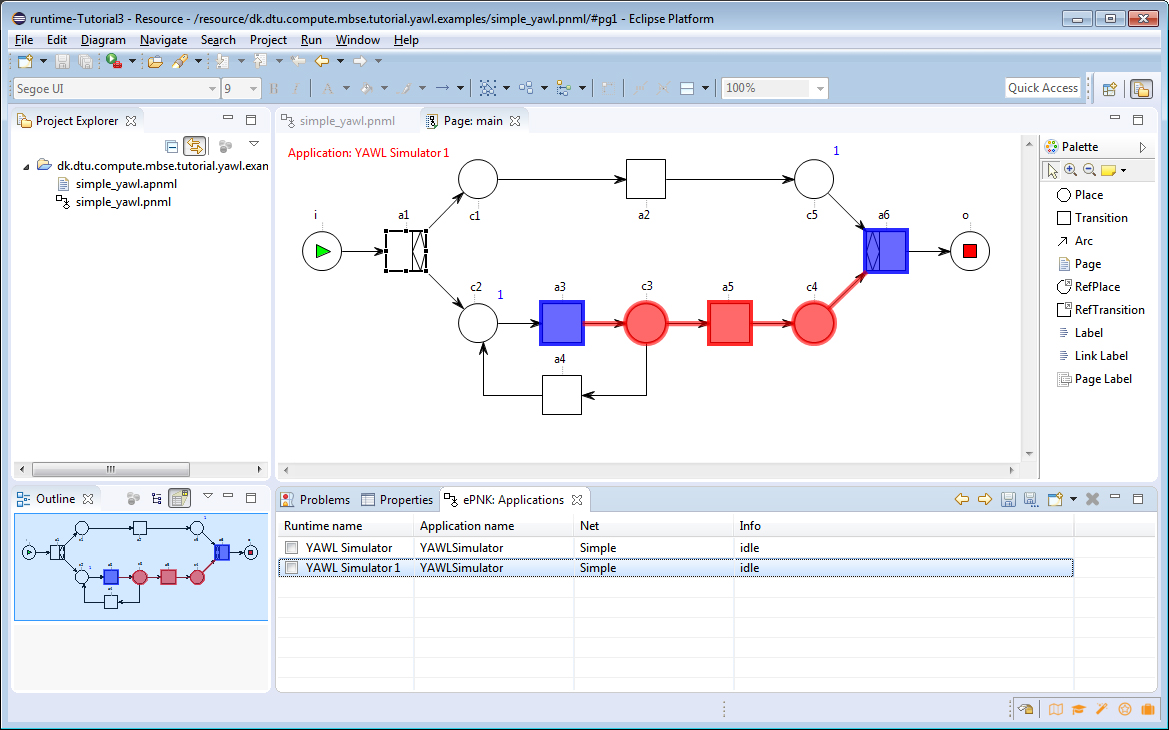
\includegraphics[scale=.29]{ePNK-yawl-sim2}}
  \caption{ePNK with two YAWL simulators running}
  \label{fig:YAWLsim2}
\end{figure}
%
A blue number at the top-right of a place indicates the number of
tokens in the current marking of the net in the active simulator; if there is
no such number at a place, the place has currently no tokens.
A blue overlay for a transition indicates that the transition is 
currently enabled. The red overlays for places, transitions and arcs indicate
a path on which a token might arrive on place {\sf c4} at the enabled
OR-join transition {\sf a6}.
This serves as a warning for the user that transition {\sf a6} should not be fired yet,
since an OR-join transition should wait for tokens that might still arrive along the
red path\footnote
{This is a subtlety of YAWL OR-joins, which we do not discuss in detail in this paper.}%
.

In Fig.~\ref{fig:YAWLsim2}, you can also see some specific features of YAWL nets.
We use this example for briefly explaining the main concepts of YAWL.
Like normal Petri nets, YAWL nets consist of \emph{places}, \emph{transitions} and
\emph{arcs}, where arcs can connect places and transitions. In YAWL, places
are called \emph{conditions}, and transitions are called \emph{actions}. YAWL
has distinguished \emph{start conditions} and  \emph{finish conditions},
which is a special attribute associated with conditions; and these conditions
are graphically distinguished by special symbols as shown for start condition
{\sf i} and finish condition {\sf o}. YAWL nets, actually, require that there
is exactly one start condition and one finish condition. Moreover, YAWL actions
can define different ways, how an action with multiple incoming arcs synchronizes
incoming tokens, called \emph{AND-}, \emph{OR-} and \emph{XOR-joins}; we call
this the \emph{join type} of the action. Likewise, a YAWL action with
multiple outgoing arcs can define different \emph{split types}, called
\emph{AND-}, \emph{OR-} and \emph{XOR-splits}, which define
how many outgoing arcs of the action should produce a token when the transition fires.
The join and split types are two attributes of an action, which also is
indicated in the graphical representation of the action. For example,
{\sf a1} is an OR-split action, and {\sf a6} is an OR-join action indicated
by the diamond symbol on the right or left side of the respective action.
YAWL nets have some additional features like \emph{reset arcs}.
But, for simplicity, our example from Fig.~\ref{fig:YAWLsim2} does not
use reset arcs.

Once a YAWL simulator application is running on a YAWL net and selected as
the active one in the ePNK \emph{application view}, the user can interact with
the simulator by double clicking on the enabled transitions. This will fire
the respective transition and then show the successor marking.
Moreover, the user can go back and forth to the previous or next marking by pressing
the backwards and forwards button in the toolbar of the \emph{application view}.
From the \emph{application view}, it is also possible to save the current state of the simulator
with the save button and to start new applications via the drop down menu, which will
show all the ePNK applications that are applicable for the net in the currently active
editor. Moreover, the user can shut down applications or load an application
from a state that was saved earlier.

\section{ePNK applications: Overview}
\label{sec:overview}

The ePNK comes already with different Petri net types and simulators for
the different net types.
% There even exists a simulator application for high-level nets, which
% animates the behaviour of a net in a virtual 3D-visualisation.
But, the main purpose of the ePNK are not the Petri net types and the applications
it comes with, but the possibility to create and plug in new Petri net types and
new applications.

Basically, an ePNK application is some additional software on top of the ePNK, which
is started on a Petri net, which can show some results or intermediate states
with some graphical overlays on top of the graphical editor of the underlying net
and interacts with the end user via these overlays and the buttons in
the ePNK application view as discussed for the YAWL simulator in Fig.~\ref{fig:YAWLsim2}.
The only limitation is that each application is associated with one Petri net
only---unless you are willing to do major programming.

Typically, your own extension of the ePNK would be done in two steps.
% First, defining a new Petri net type. This step mainly consist in defining the
% concepts of your Petri net type by a so-called \emph{Petri net type definition}
% (\emph{PNTD}), which will be discussed in more detail in Sect.~\ref{sec:yawl-pntd};
First, defining the
concepts of your Petri net type by a \emph{Petri net type definition}
(\emph{PNTD}), which is discussed in more detail in Sect.~\ref{sec:yawl-pntd};
you can also customize the graphical appearance of the elements of your Petri net type
in the graphical editor. Note that the definition of a new Petri net type
is purely syntactic: it defines which objects may or may not be in this
Petri net and how the elements may be related to each other.
The Petri net type definition does not define the semantics or the firing rule
of the new type. This would be defined along with the applications,
in particular for simulators.

If you use an existing Petri net type, either because it comes with the
ePNK or is provided by some third party, you can, of course, skip the first step. 

The second step, would be defining a new \emph{ePNK application}, which consists
of two sub-steps. The first one would be defining the runtime information of
your application, which makes up the state of the application. This is
done by defining \emph{annotations}, which is discussed in
Sect.~\ref{subsec:yawl-annot}. The second sub-step is defining handlers, which
define how the annotations of the runtime information are presented to
the end user, and which actions should be taken, when the
end user interacts with an annotation. This is discussed in
Sect.~\ref{subsec:yawl-appl}. The semantics of a Petri net type is actually
defined in these actions. 

\section{The YAWL PNTD}
\label{sec:yawl-pntd}

In this section, we briefly discuss how to define a new Petri net type. The
concepts of a Petri net type are defined by providing a class diagram\footnote
  {Technically, it is an Ecore model, which is kind of a light-weight version
   of UML class diagrams used by EMF \cite{BSM06}.}%
. This is called a \emph{Petri net type definition} (\emph{PNTD}).
Figure~\ref{fig:YAWLPNTD} shows the PNTD for YAWL nets. Note that the new concepts,
which are shown in light colour, extend the concepts from the \emph{PNML core model},
which are shown in magenta on the left-hand side and the class {\sf Attribute}.
YAWL's \emph{Conditions} are derived from \emph{Places} of the
\emph{PNML core model}.  Conditions have an additional \emph{attribute}
type, saying whether it is a \emph{normal}, a \emph{start} or a \emph{finish} place.
\emph{Actions} are derived from \emph{Transitions} of the \emph{PNML core model};
they have two additional attributes, defining the \emph{join-} and the
\emph{split-type} of the transition: these attributes can have values
\emph{AND}, \emph{XOR} and \emph{OR}. Likewise YAWL's \emph{Arcs} extend the
\emph{Arcs} from the \emph{PNML core model}: YAWL arcs have one additional
attribute defining the type of the arc, which can be \emph{NORMAL} or \emph{RESET}.

\begin{figure}[tb!!]
  \centerline{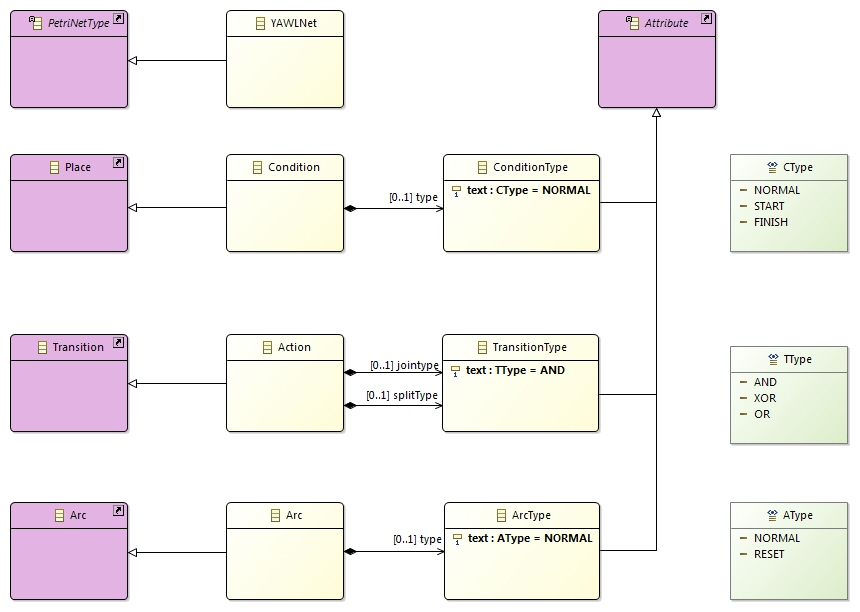
\includegraphics[scale=.35]{yawl-pntd}}
  \caption{PNTD for YAWL}
  \label{fig:YAWLPNTD}
\end{figure}

In addition to the concepts defined in the model, there are some \emph{constraints}.
Generally, constraints are used to express subtle restrictions on the combination
of objects or the legal values of attributes that would be difficult or
inconvenient to express in class diagrams. In UML, these are often expressed
in OCL.  For our example, there is a constraint saying that a YAWL net must
have exactly one start and exactly one finish place; an other constraint is
that a start place should not have incoming arcs; and a finish place should not have outgoing
arcs---and some more. In the EMF technology underlying the ePNK \cite{BSM06}, these additional
constraints can be formulated either in OCL or programmed in Java. But, we do not discuss the
technical details here. If you are interested, you can look them up in the plugin
project for YAWL nets (see Sect.~\ref{sec:techdetails}).
% technical details here. If you are interested, you can look them up in the plugin
% project for YAWL nets, which comes with the ePNK~1.2 (see Sect.~\ref{sec:techdetails});
% in this plugin, there are examples of OCL as well as Java constraints.

In contrast to earlier versions of the ePNK, which required
some minor programming, version 1.2 of the ePNK does not need any programming for
plugging in a new PNTD; the model from Fig.~\ref{fig:YAWLPNTD} and the code generated
from it by EMF \cite{BSM06} can be plugged directly into the ePNK.

In addition to the PNTD, we would also like to customize the graphical appearance
of \emph{start} and \emph{end places}, \emph{reset arcs} and the \emph{split-} and \emph{join-types}
of transitions so that they look like YAWL nets. For each
object type, we, basically, need to program a class with a method that draws the
respective object dependent on its context and its different attributes; and then,
plug these classes into the ePNK. Then, the graphical editor of the ePNK is
able to show YAWL nets as shown in Fig.~\ref{fig:YAWLsim2}. 
You will find the details in the implementation of the YAWL plugin projects
(see Sect.~\ref{sec:techdetails}).

\section{The YAWL Simulator}
\label{sec:yawl-sim}

Next, we discuss how to realize a
simulator for YAWL nets as an example of how to realize an ePNK application.

\subsection{The Annotations}
\label{subsec:yawl-annot}

The first step is to define the \emph{runtime information} of the application.
Of course, it depends on the specific application what constitutes this
\emph{runtime information}. For our YAWL simulator, this runtime
information is the current marking of the net along with the
sequence of all markings up to the current one. Technically, the runtime
information of an ePNK application is defined by \emph{annotations},
which are associated with the net itself and with the net's objects.

Figure~\ref{fig:YAWLAnnotations} shows the class diagram defining the annotations
for the YAWL simulator. This diagram consists of three parts: The two classes
{\sf PetriNet} and {\sf Object} on the left come from the \emph{PNML core model} \cite{HKea09}
and represent the Petri net and its different kinds of objects. These are
the objects which are supposed to be annotated. The classes at the top
in dark orange, represent the general annotations that are built into
the ePNK. These are extended by the annotations of a specific application,
which, in our case, are the three classes at the bottom.
%
\begin{figure}[tb!!]
  \centerline{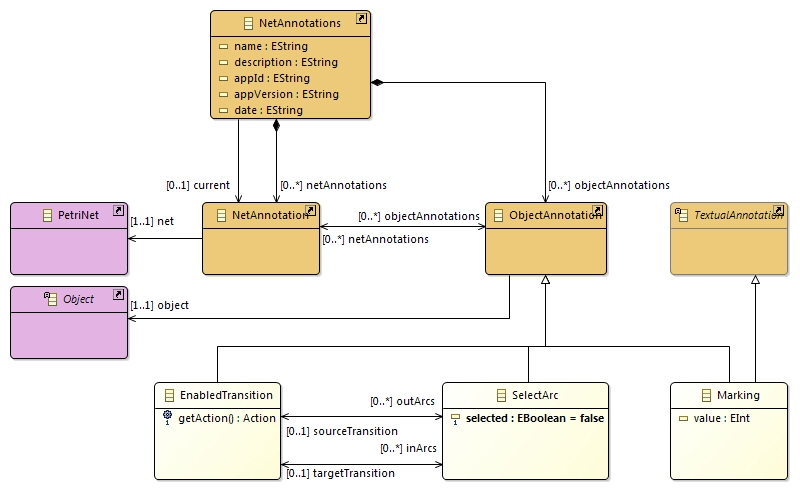
\includegraphics[scale=.35]{yawl-annotations}}
  \caption{YAWL annotations}
  \label{fig:YAWLAnnotations}
\end{figure}

Let us have a closer look at these concepts: The two concepts {\sf PetriNet}
and {\sf Object} represent \emph{Petri nets} along with their \emph{objects}: places,
transitions, and arcs; but also pages, reference transitions and reference
places. As said already, these are the objects annotations refer to.
The orange classes at the top are ePNK's built-in concepts of annotations.
An {\sf ObjectAnnotation} annotates exactly one object, which is
represented by the reference {\sf object}. Note that
a Petri net and its objects do not know anything about their annotations
at all, since applications should be detached from the net they are running
on. A {\sf NetAnnotation} refers to one
Petri net and consist of many object annotations. These constitute a specific
situation in the application at runtime; in the YAWL simulator, this would be
a marking. The class {\sf NetAnnotations}
comprises all the annotations of a running application, a sequence of net
annotations; one {\sf NetAnnotation} is pointed out as the application's
\emph{current} one, which is the one shown with labels and overlays on top
of the graphical editor of the net, when the application is active. In
our YAWL simulator, this would be the current marking.
An ePNK application is actually associated with exactly one {\sf NetAnnotations}
object, which in turn contains all the application's relevant runtime information
in its associated sequence of {\sf NetAnnotation} objects.
The interpretation of this sequence is up to the concrete application, but the
default interpretation is a sequence of net annotations. In our YAWL simulator,
it represents a sequence of markings, with one distinguished as the {\sf current}
one.
The class {\sf NetAnnotations} has some additional attributes,
which are relevant when an application---actually its state---is saved.
In particular, the {\sf appId} is used for identifying the application from
which the annotations have been saved; this is used for 
starting the same application again when the end user loads the application
from its saved state.

The three classes at the bottom of Fig.~\ref{fig:YAWLAnnotations} define the annotations
for our YAWL simulator: {\sf EnabledTransition}, {\sf SelectArc} and {\sf Marking},
which we have seen representations of in Fig.~\ref{fig:YAWLsim2} already.
Note that we do not define specific annotations for high-lighting the path of
possible tokens arriving at an OR-join here, since we can reuse
{\sf ObjectAnnotation} for this purpose, which is defined by the ePNK already.
The ePNK annotation model has an abstract class {\sf TextualAnnotation}.
An ePNK application, by default, presents annotations inheriting from
{\sf TextualAnnotation} as textual labels at the top-right of the object
in the graphical editor, showing the value of its {\sf text} or {\sf value} attribute.
In our YAWL simulator, {\sf Marking} is an example of such a textual annotation. All other 
annotations are, by default, shown as red overlays of the respective
object. But, we will see later that an application can change this.
%
The annotation {\sf SelectArc} is used for indicating which arcs of an enabled
transition can be selected by the user, and which of the arcs are currently
selected, represented by the attribute {\sf selected}. This is relevant for the
arcs of XOR-join and -split transitions and for OR-split transitions in order for
the end user to be able to select from which places tokens are to be consumed and on which
places tokens should be produced when the transition fires. To this end, the user
will be able to select a combination of arcs for the respective transition
(the selected ones shown in blue, the not selected ones shown in grey).
In order to program the logic of the arc selection, the {\sf SelectArc} annotation
is associated with the respective {\sf EnabledTransition} annotation.

Altogether, the classes from Fig.~\ref{fig:YAWLAnnotations} allow a running
simulator to store its {\sf state} with a {\sf NetAnnotations} object as its root.
We call this
the \emph{runtime information} of the simulator. Note, that this can be much
more than what is currently shown to the end user; only the {\sf current}
{\sf NetAnnotation} is shown to the end user.

Associating exactly one {\sf NetAnnotations} object with each application
makes it easy for the ePNK to save the runtime information of an application
to a file. And the ePNK can load this file again, and start the corresponding
application, since the application's id is stored as an attribute of the top-level
{\sf NetAnnotations} object. This way, a developer of an ePNK application
does not need to program anything for realizing the load and save feature
of the application. By overriding the {\sf isSavable()} method, the application
can decide whether it should be possible to save its runtime information or not.

This mechanism makes it possible to exchange the runtime information
of  applications among different tools, as long as they agree on the annotation
models, the underlying PNML core model, and on the way the instances of the annotation
model are serialized. The ePNK currently uses XMI \cite{XMI03} for this purpose.
But, it would be possible to define a dedicated XML-format that
would closely resemble the mapping of the PNML core model to XML. This way,
we have a format for interchanging analysis results of Petri nets among
different tools. Of course, this helps exchanging the information on a technical
or syntactic level only. The conceptual work of 
defining the meaning of the different annotations and devising
standard annotations for the most relevant ones would be up for
discussion in the Petri net community, which then could lead to
an extension of the ISO/IEC~15909-2 standard
\cite{ISO-IEC:15909-2-2011}.

\subsection{The Application}
\label{subsec:yawl-appl}

In addition to defining its runtime information, an application must
implement three different things: the \emph{initialization}, some
\emph{presentation handlers}, and some \emph{action handlers}.
The \emph{initialization} computes the initial net annotations that
represent the initial state (the initial marking in our case); 
the \emph{presentation handlers} define how the different
object annotations should be presented to the end user as labels or overlays
in the graphical editor, if the ePNK's default representations are not sufficient;
the \emph{action handlers} define what should happen when the end user interacts
with an annotation (or actually its presentation) in the graphical editor.

Separating the definition of the runtime information, the presentation
handlers and the action handlers in applications follows the architectural
pattern of \emph{model-view-controller} (\emph{MVC}).

Here, we cannot discuss all the details of implementing the action handlers
and the presentation handlers, for which you can have a look into the YAWL plugins
(see Sect.~\ref{sec:techdetails}). But, we give a brief overview here. The YAWL simulator
has two action handlers: one for firing the transition when the end user double clicks on
an enabled transition annotation, and one for selecting or unselecting
an arc when the user clicks on a select arc annotation. The \emph{enabled transition}
handler, basically, adds a new net annotation to the state of the simulator with the
annotations representing the new marking, and it makes this new net annotation the
current one. This is where the actual semantics of YAWL is implemented.
The \emph{select arc} handler, basically, toggles the {\sf selected}
attribute taking the semantics of the respective split or join into account.

A presentation handler, basically, returns an overlay figure for the 
graphical figure that represents the annotated object in the graphical editor. In our
case, it returns a blue overlay for an enabled transition and, dependent on the
{\sf selected} attribute of the {\sf SelectArc} annotation, a blue or grey overlay for
the annotated arc.
For all other annotations, ePNK's default presentation handler kicks in, returning
a red overlay.

\section{Discussion}
\label{sec:discussion}

In the previous sections, we have discussed the main steps of realizing
YAWL nets and a simulator for them. In both parts, models
played a major role: the concepts of YAWL nets are represented in the model
shown in Fig.~\ref{fig:YAWLPNTD}; likewise, the model of the runtime
information is shown in Fig.~\ref{fig:YAWLAnnotations}.
Based on the model of the runtime information, an ePNK application is
realized following the MVC-pattern: the runtime information is represented
in the model as annotations, the presentation handlers define how the annotations
should be shown on top of the net in a graphical editor, and the action handlers
define the controllers. 

Defining the runtime information of an application by a model has an additional
advantage: It allows the ePNK to generically save and load the state of the
application without any additional programming by the developer.
This could be the basis for an interchange format of analysis results,
as  discussed in the end of Sect.~\ref{subsec:yawl-annot}.

\begin{figure}[tb!!]
  \centerline{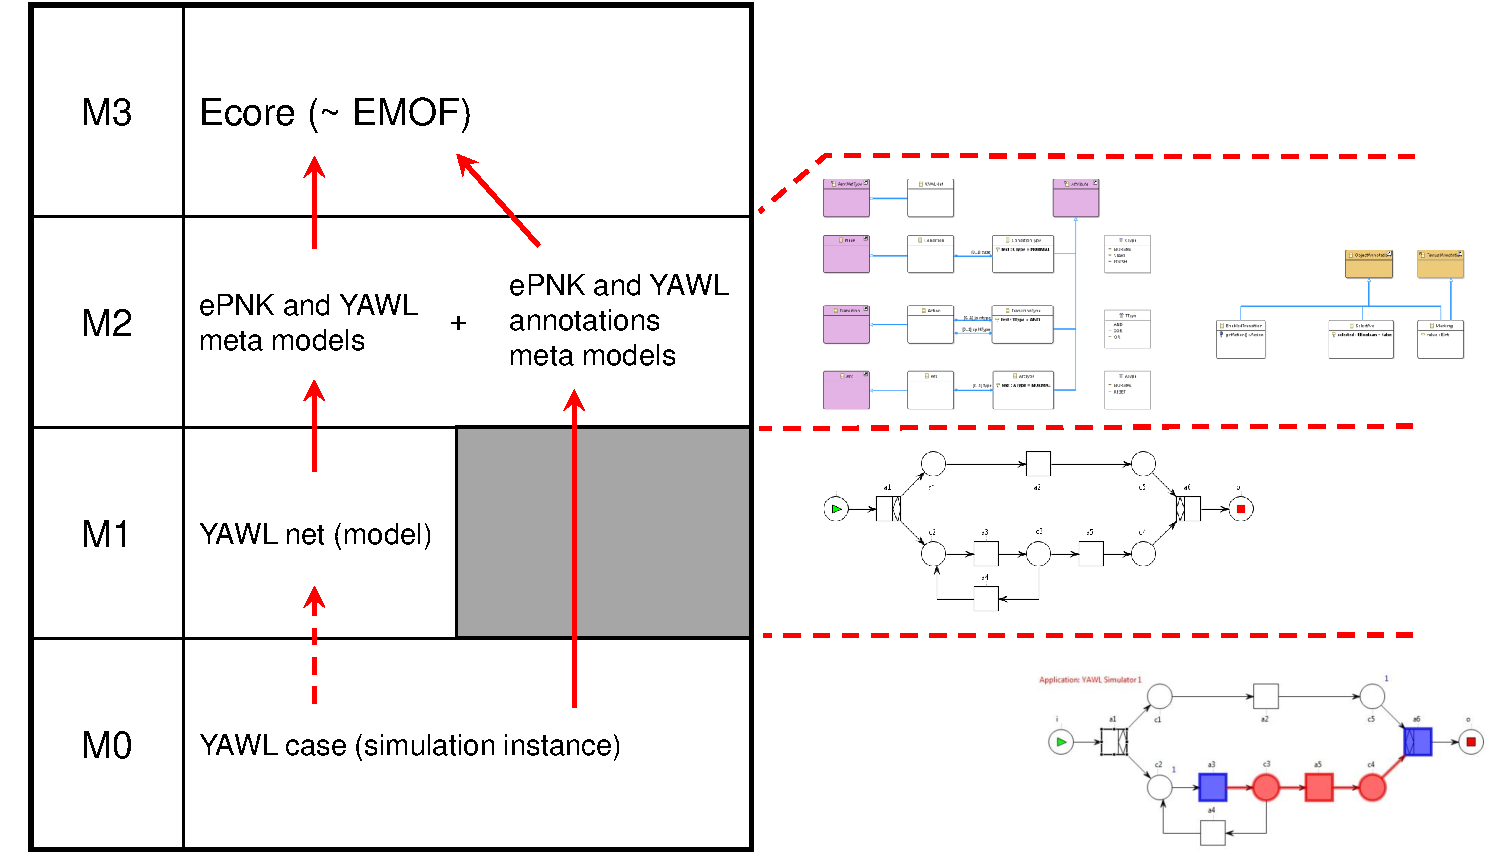
\includegraphics[scale=.48]{MOF-YAWL}}
  \caption{MOF levels: YAWL nets and simulator}
  \label{fig:MOF-YAWL}
\end{figure}

Figure~\ref{fig:MOF-YAWL} gives an overview of the different models and
meta models involved in defining Petri nets and the annotations used for 
applications, as well
as the different instances of these models. It shows the models, meta models and
instances on the levels of the so-called MOF hierarchy \cite{MOF05}. On level M2,
there are the PNML core model, which is also the meta model of the ePNK, and
the meta model for the PNTD of YAWL---which together define what YAWL nets
are. On level M1, there are the
YAWL nets which are instances of the meta models on M2, which is indicated
by the red arrow. On level M2, there are also the meta models of the runtime
information (annotations) of the applications. An instance of that meta model would
be a running simulation, a \emph{case} of a YAWL net, with its current marking;
this is shown on level M0.
Note that, conceptually, a case is an instance of a YAWL net on level M1,
indicated by the dashed red arrow; but technically, a YAWL case is an instance
of the annotation meta models on level M2. Therefore, the \emph{technical instance}
jumps one level. Note, in particular, the difference between the solid red arrows that
represent a \emph{technical is instance} relation and the dashed red arrow that
represents a \emph{conceptual is instance} relation.
On level M3, is the meta meta model defining the concepts of Ecore diagrams,
which are used to formulate the PNTD of YAWL and the annotations for the
YAWL simulator.

\section{Related work and limitations}
\label{sec:related-work}

The ePNK was developed for fully exploiting the concepts of PNML \cite{HKea09} and,
in particular, the concept of \emph{Petri net type definitions}. There are many
tools that support PNML in some form or the other (a few of them are listed on the
PNML Home page \cite{PNMLURL09}). But, most tools support only a fixed set of Petri
net types, and it is not easily possible to define a new one. The PNML Framework
\cite{DBLP:conf/apn/HillahKPT10} is a notable exception, in that it is made for defining
new Petri net types by using PNTDs. The limitation of the PNML Framework, however, is
that the complete code of the PNML Framework needs to be recompiled for
a new PNTD. The ePNK allows plugging in new PNTDs without recompiling the
ePNK itself. Moreover, the PNML Framework does not have a graphical editor for Petri
nets.

There are several Petri net and Petri net related tools, which allow to plug in
new functionality, which we could call applications in our context. Some examples are
CPN Tools \cite{CPNHome}, ProM \cite{PRoMURL}, and Renew \cite{DBLP:conf/apn/KummerWDSKMRV04}.
ProM is explicitly made for plugging in new process mining techniques and also
allows implementing new notations, but not in the sense of PNTDs. CPN Tools and
Renew mostly use a fixed Petri net type (coloured nets and reference nets, respectively).
But they allow to plug in new applications. And it is possible to give feedback
in the respective graphical editor.

So, the ePNK with its plugin mechanism for easily defining new Petri net types
as well as applications fills a very special niche: it is easy to define
an application on a new or slightly extended version of Petri nets. Concerning
the definition of new notations or new Petri net types, the limitation of
the ePNK is that the new notation needs to be a ``kind of a Petri net'' since
it needs to extend the PNML core model by design:
so the new notation should have two cardinal types of nodes (place-like and transition-like
nodes); of course, the ePNK could be
abused, since it is possible to squeeze in many different kinds of nodes and arcs
by additional attributes for places and transitions and arcs. But, we would 
consider that to be artificial. The example of YAWL nets, however, shows that notations
that have nodes of many different kinds and with attributes can easily represented
as a PNTD, if they fall into two major categories.

What concerns applications, the limitations are that the main information of
an application is supposed to be shown on top of the graphical nets. Of course,
an application can implement additional views---an example would be the
ePNKs simulator for high-level nets, which has a view for the complete history of
the simulation. But, that requires much more programming and defies to some
extent the original idea of the ePNK.

We believe that within these limits, the ePNK will be of use for people
who would want to quickly experiment with an idea for a new Petri net type
or a simple application. They would get a graphical editor and the graphical
presentation of results of their application and the interaction with the end user,
basically, for free.
For us, the ePNK came in handy when we needed a notation
for defining the life-cycle of objects in the context of the \emph{Event Coordination
Notation} (\emph{ECNO}) \cite{Kin14a}: We could very quickly define ECNO nets by a
Petri net type definition for the ePNK. From these models plus ECNO's coordination model,
running software could be generated fully automatically. 


\section{Technical details}
\label{sec:techdetails}

The ePNK is realized as an extension of Eclipse. In order to install it on your
computer, you need to install Java and Eclipse\footnote
{If you intend to use the ePNK for developing own Petri net types or
 applications, it is recommended to install the ``Eclipse Modeling Tools''
 package of Eclipse.}%
. Then, you can install the ePNK
from inside Eclipse (Help$\rightarrow$Install New Software $\ldots$). Version~1.2
of the ePNK can be installed by creating a new update site 
\url{http://www2.compute.dtu.dk/~ekki/projects/ePNK/1.2/update/} and then
selecting all ePNK features. The update site includes a ``YAWL net type,
graphical extension and simulator'' feature, which includes all YAWL extensions
discussed in this paper as well as some YAWL example nets.

These projects come with the complete source code, so that you can look up the
technical details and implementation issues, which we could not discuss in this
paper. To this end, open the ``Plug-ins'' view of Eclipse
(Window$\rightarrow$Show View$\rightarrow$Other$\ldots$)
and, in this view, select all YAWL projects, which
have the prefix {\sf dk.dtu.compute.mbse.tutorial.yawl}; right-click on them
and select Import As$\rightarrow$Source Project. After that, you will
have five new projects in your Eclipse workspace.

The project {\sf dk.dtu.compute.mbse.tutorial.yawl.examples} contains
three PNML files with YAWL nets---among others, the file {\sf simple\_yawl.pnml},
which is the example shown in Fig.~\ref{fig:YAWLsim2}. You can open it by double-clicking
on it. Note that the file opens in the ePNK's tree editor; you can fold out the
document's objects until the pages appear, and then open the graphical editor
by double-clicking on the page. Then, you should open the  ``ePNK: Applications''
view as discussed above for the ``Plug-ins'' view.  From there, you can start
a new YAWL simulator via the drop down menu; from there, you can also load the
example simulation ({\sf simple\_yawl.apnml}) discussed in this paper by
``Load Application'' and then navigate back and forth in this simulation.

For looking up technical details of the implementation, you can look into the
other projects: {\sf dk.dtu.compute.mbse.tutorial.yawl} contains the definition
of YAWL nets. {\sf dk.dtu.compute.mbse.tutorial.yawl.graphics} implements
the custom graphics for YAWL nets, and {\sf dk.dtu.compute.mbse.tutorial.yawl.simulator}
implements the YAWL simulator. The last project, {\sf dk.dtu.compute.mbse.tutorial.yawl.\ edit}
contains automatically generated code only.



\begin{comment}
\section{Additional features of version~1.2}
\label{sec:new-features}

Since the initial release and publication of the ePNK \cite{Kin11d} at Petri Nets 2011,
and even with respect to the major release of version 1.0 in 2012 \cite{Kin12c}, many new
features have been added to the ePNK, and several bugs have been fixed.

Some of the main extensions with respect to version~1.0 are:
\begin{itemize}
  \item Originally, implementing a new Petri net type required some minor programming. In
        version~1.2, an Ecore model and the code generated from it is actually enough to
        create a Ecore model for the new PNTD; from this model, the plugin for the ePNK can be generated
        automatically by an action. Moreover, the names of the extended classes for the
        respective Petri net objects do no
        longer need to be the same as in the PNML core model, and Petri net types
        can---without doing any extra programming---be derived from one or more existing types.
        
  \item ePNK applications are now explicitly known and controlled by the ePNK; the
        state of an application can be saved and loaded again, and the implementation
        of an application follows the MVC-pattern now.
        
  \item For types with many labels for its objects, there is a user action which
        automatically adds all default labels to an object of a net.
\end{itemize}

New features:
  - no programming for PN types at all (even when classes for types are not named
    Place, Transition and Arc anymore, which needed programming before)
  - advanced support of applications and application view
  - model view controller structure for applications
  - loading and saving the state of an application
  - advanced derivation of types of places, transitions, arcs and other
    object types, when a net type is derived from one ore more net types
    (no programming even when combining types)
  - action that adds all default labels to a net object (equally distributed around it)
\end{comment}

\section{Conclusion}
\label{sec:conclusion}

By the example of YAWL nets and the YAWL simulator, we have discussed the
main idea of ePNK applications and how they are realized based on the ePNK's
annotation model. Like the definition of YAWL nets themselves, the
runtime information of the simulator is defined by a model as an extension
of ePNK's annotations model. Using models not
only for defining new types, but also for representing the runtime information,
makes it easier to load and save the state of applications in a uniform and
generic way. This could actually be used as a basis for a generic but yet
extensible standard interchange format for analysis results of Petri nets as
an extension of PNML \cite{HKea09,ISO-IEC:15909-2-2011}. 

\begin{comment}
In this paper, we could not provide all the technical details of realizing PNTDs and
applications for the ePNK. For details and a tutorial, we refer to a revised manual
of version~1.2 of the ePNK, which will be published shortly \cite{Kin17c}.
\end{comment}

% {\small
% \paragraph*{Acknowledgements}

% }

% \bibliographystyle{splncs}
% \bibliography{all}

\begin{thebibliography}{10}

\bibitem{HKea09}
Hillah, L., Kindler, E., Kordon, F., Petrucci, L., Treves, N.:
\newblock A primer on the {Petri Net Markup Language} and {ISO/IEC 15909-2}.
\newblock In Jensen, K., ed.: $10^{th}$ Workshop on Coloured Petri Nets (CPN
  09). (2009)  101--120

\bibitem{ISO-IEC:15909-2-2011}
ISO/IEC:
\newblock {Systems and software engineering -- High-level Petri nets -- Part 2:
  Transfer format, International Standard ISO/IEC 15909-2:2011} (2011)

\bibitem{Kin11d}
Kindler, E.:
\newblock The {ePNK}: {An} extensible {Petri} net tool for {PNML}.
\newblock In: Applications and Theory of Petri Nets - $32^{nd}$ International
  Conference, Proceedings. Volume 6709 of LNCS., Springer (2011)  318--327

\bibitem{Kin12c}
Kindler, E.:
\newblock The {ePNK}: A generic {PNML} tool - {Users' and Developers' Guide}
  for version 1.0.0.
\newblock Technical Report IMM-Technical Report-2012-14, DTU Informatics, Kgs.
  Lyngby, Denmark (2012)

\bibitem{vAtH05}
van~der Aalst, W., ter Hofstede, A.:
\newblock {YAWL}: Yet another workflow language.
\newblock Information Systems \textbf{30}(4) (2005)  245--275

\bibitem{BSM06}
Budinsky, F., Steinberg, D., Merks, E., Ellersick, R., Grose, T.J.:
\newblock Eclipse Modeling Framework. 2nd edn.
\newblock The Eclipse Series. Addison-Wesley (2006)

\bibitem{XMI03}
{OMG}:
\newblock {XML} metadata interchange ({XMI}) specification, version 2.0.
\newblock Technical Report formal/03-05-02, The Object Management Group, Inc.
  (2003)

\bibitem{MOF05}
{OMG}:
\newblock {Meta Object Facility} ({MOF}) specification, version 1.4.1.
\newblock Technical Report formal/05-05-05, The Object Management Group, Inc.
  (2005)

\bibitem{PNMLURL09}
{PNML team}:
\newblock {PNML}.org: The {Petri Net Markup Language} home page.
\newblock \url{http://www.pnml.org/}

\bibitem{DBLP:conf/apn/HillahKPT10}
Hillah, L.M., Kordon, F., Petrucci, L., Tr{\`e}ves, N.:
\newblock {PNML Framework}: An extendable reference implementation of the
  {Petri Net Markup Language}.
\newblock In Lilius, J., Penczek, W., eds.: Petri Nets. Volume 6128 of Lecture
  Notes in Computer Science., Springer (2010)  318--327

\bibitem{CPNHome}
{CPN Tools}:
\newblock Home page.
\newblock \url{http://cpntools.org/}

\bibitem{PRoMURL}
PRoM tools:
\newblock Home page.
\newblock \url{http://www.promtools.org/doku.php}

\bibitem{DBLP:conf/apn/KummerWDSKMRV04}
Kummer, O., Wienberg, F., Duvigneau, M., Schumacher, J., K{\"o}hler, M., Moldt,
  D., R{\"o}lke, H., Valk, R.:
\newblock An extensible editor and simulation engine for {Petri} nets: Renew.
\newblock In Cortadella, J., Reisig, W., eds.: ICATPN. Volume 3099 of Lecture
  Notes in Computer Science., Springer (2004)  484--493

\bibitem{Kin14a}
Kindler, E.:
\newblock Coordinating interactions: The {Event Coordination Notation}.
\newblock Technical Report DTU Compute Technical Report 2014-05, DTU Compute,
  Kgs. Lyngby, Denmark (2014)

\end{thebibliography}


\end{document}
